\section{Dataset Collection}

We use Stack Exchange Data
Explorer\footnote{\texttt{https://data.stackexchange.com/stackoverflow/query/new}}
and construct a custom SQL query on the Stack Overflow data. The query could be
found under \texttt{source\_code/raw\_data/query.sql}.

The query satisfies the three requirements:

\begin{itemize}
    \item \texttt{\ldots select top 500} means that we are collecting at least
    500 threads.
    \item \texttt{\ldots Tags like \textquotesingle{}\%python\%\textquotesingle{}}
    means that we are collecting threads tagged \texttt{python}, discussing the
    Python programming language.
    \item \texttt{\ldots where AnswerCount >= 1} means we are collecting
    threads with at least 1 question and 1 answer.
\end{itemize}

The dataset contains 500 questions and 1254 answers, an average of 2.508 answers
per question. The distribution of answers is shown in Figure~\ref{ans-dist}.

\begin{figure}[htp]
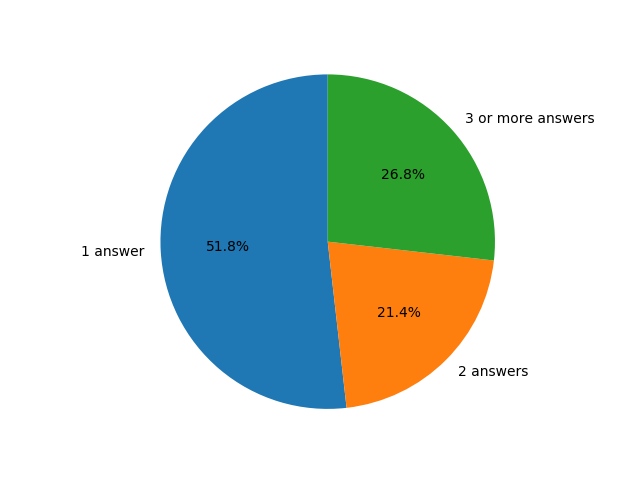
\includegraphics[width=0.85\linewidth]{no_ans_per_qn}
\caption{Distribution of answers}\label{ans-dist}
\end{figure}

\section{Dataset Analysis and Annotation}

\subsection{Stemming}

We use NLTK~\cite{nltk} to stem the dataset; the implementation is in
\texttt{source\_code/stem\_and\_pos.py}.
Prior to stemming, HTML tags and punctuations are removed using regular
expressions, and stopwords such as ``a'', ``of'' and ``the'' are also
excluded, using the stopwords corpus available in NLTK
(\texttt{nltk.corpus.stopwords.words\\('english')}); this ensures that we are
getting the most meaningful words from the dataset. A Porter stemmer is 
used (\texttt{nltk.stem.\\PorterStemmer().stem()}; the top 20 words before
and after stemming are in Table~\ref{stem}.

\begin{table}[htp]
\caption{Top 20 words before and after stemming}\label{stem}
\begin{tabu}{X[1,l]X[4,l]|X[4,l]X[10,l]}
    \textbf{} & \textbf{Before stemming} &
    \textbf{After stemming} & \textbf{Original words} \\
    \midrule
    1 & I & I & I \\
    2 & Python & use &
    used, using, use, Use, useful, uses, Using, Usings \\
    3 & import & python &
    Python, Pythons, python, Pythonic, pythonic, pythons, pythonicity \\
    4 & use & import &
    import, imports, important, imported, Imported, importing, Import \\
    5 & 1 & 1 & 1 \\
    6 & def & def & def \\
    7 & You & return & 
    return, returns, returning, Returning, Returns, returned \\
    8 & return & file &
    files, file, File \\
    9 & using & tri &
    trying, tried, try, Try, tries, Trying, Tried \\
    10 & print & print &
    print, prints, printing, printed, Prints \\
    11 & like & you & You \\
    12 & code & like & 
    like, likes, likely, liked, Like \\
    13 & gtgtgt & code &
    code, coding, CODE, Code, Codes \\
    14 & class & list &
    list, Lists, lists, LIST, listing, List, listed \\
    15 & python & class &
    class, Class, classes, Classes \\
    16 & 2 & gtgtgt &
    gtgtgt, gtgtgts \\
    17 & list & function &
    function, functions, functionality, functional, Function \\
    18 & 3 & want &
    want, wanting, wants, wanted \\
    19 & want & valu &
    values, value, Values, Value \\
    20 & x & 2 & 2
\end{tabu} 
\end{table}

Using Porter Stemming algorithm, majority of the words retained their
semantic meaning after stemming. However, there were some irregularities
which caused the stemming to be incorrect.

Firstly in row 4, the word ``important'' was stemmed to the word ``import''.
This is an example of derivational suffix which not only changes the word class,
but also changes the semantic meaning of the word. Porter Stemming algorithm was
not able to capture the irregularity in this scenario. 

Looking at row 9, original words were variations of the word ``try''. After
stemming, all of them were stemmed to a single word, ``tri''. This word had a
meaning of ``three'' which was clearly different from ``try''. Porter Stemming
algorithm had mistakenly treated all variations of ``try'' as ``tri''.

Lastly, at row 19, variations of ``value'' were stemmed to the word ``valu''.
The word ``valu'' is not a proper English word. Porter Stemming algorithm had
generated a word that does not exist in the English dictionary.

\subsection{POS Tagging}

We picked 10 sentences at random and applied POS tagging, using NLTK 
(\texttt{nltk.pos\_tag\_sents(tokenized\_data)}, the implementation is
also in \texttt{source\_code/stem\_and\_pos.py}).
The results are in Table~\ref{pos}; the following discussion would be
focusing on the wrongly tagged tokens and the ability to handle some
tokens with different classes.

The word ``rough'' could be tagged under three classes --- verb, noun,
adjective. In the second sentence, it was tagged as noun. However, looking at
the sentence as a whole, the word was used to modify the word ``definition''.
It should be tagged as an adjective (JJ), similar to the word ``succinct''.

In the third sentence, the token ``\,`\,'' was a mistake by author of the post. It
should have been ``\,'s\,''. The tagger was able to identify this error and
correctly tagged it as possessive ending (POS). In addition, ``\,'s\,'' in sentence
4 has a different meaning from possessive ending; it is meant to be a short
form for ``is'' and thus, should be tagged as a verb (VBZ). The tagger is also
able to handle this difference.

Looking at the fifth sentence, due to the tokenizer,
``{[}\textbackslash{}u0000-\textbackslash{}uFFFF{]}'' was splitted into
three tokens: ``['',
``\textbackslash{}u0000-\textbackslash{}uFFFF'', ``]'', causing each token to
be tagged separately and incorrectly. It would make more sense to think of
``{[}\textbackslash{}u0000-\textbackslash{}uFFFF{]}'' as a single noun.
The tagger was applied again on the sentence after manually forcing
``{[}\textbackslash{}u0000-\textbackslash{}uFFFF{]}'' to be a single token,
resulting in the correct tagging of noun (NN). This shows the importance of a
good tokenizer.

The words ``mod\_wsgi'' and ``apache'' in the seventh sentence were tagged as
noun (NN). The actual tag should be noun (NNP). However, in many cases, the
tagging of an NNP to an NN should not affect the application adversely. Thus,
this type of error was generally acceptable.

\begin{table}[htp]
\caption{POS Tagging}\label{pos}
\begin{tabu}{X[0.12,l]X[1,l]X[2,l]}
    & \textbf{Sentence} & \textbf{POS Tagging} \\
    \midrule
    1 & You are being tricked by Python's representation of the result
    string. &
    (You,PRP), (are,VBP), (being,VBG), (tricked,VBN), (by,IN), (Python,NNP),
    ('s,POS), (representation,NN), (of,IN), (the,DT), (result,NN), 
    (string,NN), (.,.) \\
    2 & I like this rough, succinct definition: A function that can refer to 
    environments that are no longer active. &
    (I,PRP), (like,VBP), (this,DT), (rough,NN), (,,,), (succinct,JJ),
    (definition,NN), (:,:), (A,DT), (function,NN), (that,WDT), (can,MD),
    (refer,VB), (to,TO), (environments,NNS), (that,WDT), (are,VBP), (no,DT),
    (longer,RBR), (active,JJ), (.,.) \\
    3 & Isn't that what Anders' second example does? &
    (Is,VBZ), (n't,RB), (that,IN), (what,WP), (Anders,NNP), (',POS),
    (second,JJ), (example,NN), (does,VBZ), (?,.) \\
    4 & There's nothing that will automatically do what you want. & 
    (There,EX), ('s,VBZ), (nothing,NN), (that,WDT), (will,MD),
    (automatically,RB), (do,VB), (what,WP), (you,PRP), (want,VBP), (.,.) \\
    5 & Use a subrange of [\textbackslash{}u0000-\textbackslash{}uFFFF] for
    what you want. & 
    (Use,VB), (a,DT), (subrange,NN), (of,IN), ([,JJ),
    (\textbackslash{}u0000-\textbackslash{}uFFFF,JJ), (],NN),
    (for,IN), (what,WP), (you,PRP), (want,VBP), (.,.) \\
    6 & Tom says it all really. &
    (Tom,NNP), (says,VBZ), (it,PRP), (all,DT), (really,RB), (.,.) \\
    7 & I have been sold on mod\_wsgi and apache rather than in mod\_python. &
    (I,PRP), (have,VBP), (been,VBN), (sold,VBN), (on,IN), (mod\_wsgi,NN),
    (and,CC), (apache,NN), (rather,RB), (than,IN), (mod\_python,NNS), (.,.) \\
    8 & This topic is covered in Django tutorials. &
    (This,DT), (topic,NN), (is,VBZ), (covered,VBN), (in,IN), (Django,NNP),
    (tutorials,NNS), (.,.) \\
    9 & The single * means that there can be any number of extra positional
    arguments. &
    (The,DT), (single,JJ), (*,NN), (means,VBZ), (that,IN), (there,EX), (can,MD),
    (be,VB), (any,DT), (number,NN), (of,IN), (extra,JJ), (positional,JJ),
    (arguments,NNS), (.,.) \\
    10 & I found Learning Python really good. &
    (I,PRP), (found,VBD), (Learning,NNP), (Python,NNP), (really,RB), (good,JJ),
    (.,.) \\    
\end{tabu} 
\end{table}

\subsection{Token Definition and Annotation}

From the 1754 posts we have extracted from Stack Overflow, 100 posts were
chosen at random and manually annotated to indicate individual tokens. The
``random'' selection of posts uses a pseudo-random algorithm with a fixed seed
(implemented in \texttt{source\_code/\\dataset.py} at function
\texttt{choose\_random\,()}) so it can be reproduced exactly each time,
given that the seed used is the same.

In the context of this project, ``token'' refers to phrases, words or
characters which can be considered as a single unit of semantic information.
Tokens cannot and should not be split further, as it would result in the loss
and/or the distortion of the information they carry. For example, we have
defined file paths and URLs as a single token, as they will lose their meaning
when split up into individual parts by more conventional tokenizers.
Table~\ref{tok} shows examples taken from the 100 tagged posts which illustrate
the rules we have used to define our tokens.

\onecolumn
\begin{table}
\caption{Some special tokenizations}\label{tok}
\begin{tabu}{X[5,l]X[5,l]X[2,l]}
    \textbf{Phrase} & \textbf{Tokens} &
    \textbf{Number of tokens} \\
    \midrule
    <p></p> && 0 \\
    <code>This is a token</code> &
    ``<code>This is a token</code>'' & 1 \\
    <a href=``https://abcxyz.com/we\_love\_nlp.py''>hello world!</a> &
    ``Hello'', ``world'', ``!'' & 3 \\
    https://abcxyz.com/we\_love\_nlp.py &
    ``https://abcxyz.com/we\_love\_nlp.py'' & 1 \\
    ``This is not a token'' &
    ``\,``\,'', ``This'', ``is'', ``not'', ``a'', ``token'', ``\,''\,'' & 7 \\
    Don't & ``Do'', ``n't'' & 2 \\
    I've & ``I'', ``\,'ve\,'' & 2 \\
    we're & ``We'', ``\,'re\,'' & 2 \\
    he'll & ``He'', ``\,'ll\,'' & 2 \\
    I'd & ``I'', ``\,'d\,'' & 2 \\
    I'm & ``I'', ``\,'m\,'' & 2 \\
    PHP's & ``PHP'', ``\,'s\,'' & 2 \\
    one1 & ``one1'' & 1 \\
    \{\% url `view' obj.id \%\} &
    ``\{\% url `view' obj.id \%\}'' & 1 \\
    {[}\% url `view' obj.id \%{]} &
    ``[\% url `view' obj.id \%]'' & 1 \\
    (how are you) &
    ``('', ``how'', ``are'', ``you'', ``)'' & 5 \\
    length-2 & ``length-2'' & 1 \\
    1/sqrt & ``1'', ``/'', ``sqrt'' & 3 \\
    Test\_Rbf & ``Test\_Rbf'' & 1 \\
    \$interpolateProvider & ``\$interpolateProvider'' & 1 \\
    \_test & ``\_test'' & 1 \\
    test\_test & ``test\_test'' & 1 \\
    test\_test\_ & ``test\_test\_'' & 1 \\
    techniques --- and & ``techniques'', ``-'', ``and'' & 3 \\
    get\,() & ``get\,()'' & 1 \\
    object.method\,(arg) & ``object.method\,(arg)'' & 1 \\
    object.attribute & ``object.attribute'' & 1 \\
    /unixfile/path/file.txt & ``/unixfile/path/file.txt'' & 1 \\
    /.. & ``/..'' & 1 \\
    /. & ``/.'' & 1 \\
    .. & ``..'' & 1 \\
    . & ``.'' & 1 \\
    C:\textbackslash{}Program Files (x86)\textbackslash{}IE\textbackslash{}
    & ``C:\textbackslash{}Program Files (x86)\textbackslash{}IE\textbackslash{}''
    & 1 \\
    D:\textbackslash{} & ``D:\textbackslash{}'' & 1 \\
    C\@: & ``C'', ``:'' & 2 \\
    \ldots & ``\ldots'' & 1 \\
\end{tabu}
\end{table}
\twocolumn

\section{Tokenizer}

We make use of multiple regular expressions (regexes) to tokenize our Stack
Overflow dataset. Five different regexes --- TAG\_REG, CODE\_REG, URL\_FILE\_REG,
EXCEPTION\_REG and TOK\_REG --- are utilised; Figure~\ref{img:tok} outlines the
tokenizer implementation given a string of text.

\begin{figure}[htp]
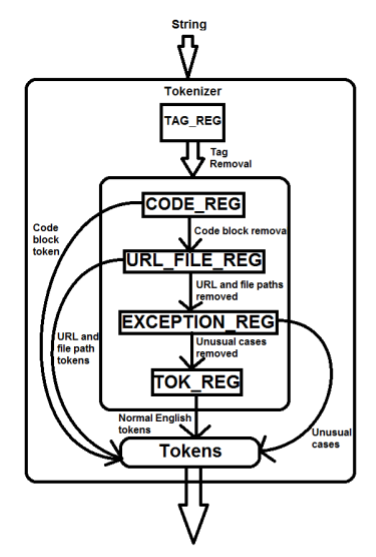
\includegraphics[width=0.9\linewidth]{tokenizer}
\caption{Tokenizer implementation}\label{img:tok}
\end{figure}

The implementation is given in \texttt{source\_code/tokenizer.py} under function
\texttt{tokenize\_v2\,()}.
TAG\_REG removes the html tags in the string, while CODE\_REG takes an entire code
block as a token. URL\_FILE\_REG then identifies the URLs and file paths (both Unix
and Windows) from the string. EXCEPTION\_REG identifies the tokens which are not
found in the English language (some examples are in Table~\ref{tok}). Finally,
TOK\_REG tokenizes the conventional English language words.

We have also written another function, \texttt{evaluate\,()} to evaluate a
tokenizer output against its ground truth (by calculating the length of the
longest common subsequence between the two lists), and output precision, recall
and F1 score.

To verify the correctness of our tokenizer, a testing script is written
(\texttt{source\_code/test.py}). This script asserts the tokenizer for given
test strings against expected tokenizer outputs (for instance,
\texttt{tokenize\_v2(`hello world')} against \texttt{[`hello', `world']}), allowing us to identify wrong cases to iteratively improve the tokenizer.
At the end of testing, the number of errors will be returned; the current
implementation is expected to pass all tests.

On the 100-post annotated dataset, the tokenizer achieves a precision of 97.2\%,
a recall of 97.6\% and an F1 score of 97.4\%.

\section{Further Analysis}

\subsection{Irregular Tokens}

We use the tokenizer in the previous section to tokenize all 1754 posts in our
dataset (the code is in \texttt{source\_code/main.py}, function
\texttt{tokenize\_dataset\,()}). The top 20 non-English tokens are summarised
in Table~\ref{non-eng}.

\begin{table}[htp]
\caption{Top 20 non-English tokens in the dataset}\label{non-eng}
\begin{tabu}{X[0.5,c]X[2,l]X[2,l]}
    & \textbf{Irregular Tokens} & \textbf{(Morphological) Forms} \\
    \midrule
    1 & Django & Django, django \\
    2 & app & app, apps, App, Apps \\
    3 & etc & etc \\
    4 & e.g. & e.g., e.g \\
    5 & dict & dict, dicts \\
    6 & HTML & HTML, html \\
    7 & regex & regex, regexes \\
    8 & csv & csv, CSV \\
    9 & i.e. & i.e., i.e \\
    10 & API & API, APIs \\
    11 & enum & enum, enums \\
    12 & GUI & GUI, GUIs \\
    13 & Java & Java, java \\
    14 & url & url, urls, URL, URLs \\
    15 & numpy & numpy, Numpy, NumPy \\
    16 & OS & OS, OSes \\
    17 & lt & lt \\
    18 & \_\_init\_\_.py & \_\_init\_\_.py \\
    19 & lxml & lxml, LXML \\
    20 & config & config, configs \\
\end{tabu}    
\end{table}

\subsection{POS Tagging}

We choose 10 sentences containing at least one of the tokens above and
perform POS tagging on them using NLTK, after running the sentences
through our own tokenizer. The results are in Table~\ref{irre}.

\begin{table}[htp]
\caption{POS Tagging of sentences with irregular tokens}\label{irre}
\begin{tabu}{X[0.2,l]X[1,l]X[2,l]}
    & \textbf{Sentence} & \textbf{POS Tagging} \\
    \midrule
    1 &
    I'm using Google App Engine and Django templates. &
    (I,PRP), ('m,VBP), (using,VBG), (Google,NNP), (App,NNP),
    (Engine,NNP), (and,CC), (Django,NNP), (templates,NNS), (.,.) \\
    2 & 
    This means it has a somewhat steep learning curve unless you are
    already familiar with libcurl's C API. &
    (This,DT), (means,VBZ), (it,PRP), (has,VBZ), (a,DT), (somewhat,RB),
    (steep,JJ), (learning,VBG), (curve,NN), (unless,IN), (you,PRP),
    (are,VBP), (already,RB), (familiar,JJ), (with,IN), (libcurl,NN),
    ("'s", POS), (C,NNP), (API,NNP), (.,.) \\
    3 & 
    Most usages of xrange, generators, etc are over static size,
    small datasets. & 
    (Most,JJS), (usages,NNS), (of,IN), (xrange,NN), (,,,), (generators,NNS),
    (,,,), (etc,FW), (are,VBP), (over,IN), (static,JJ), (size,NN), (,,,),
    (small,JJ), (datasets,NNS), (.,.) \\
    4 & 
    You can define some class variables, e.g.
    <code>refQtyA = ````qtyA''''</code>. & 
    (You,PRP), (can,MD), (define,VB), (some,DT), (class,NN), (variables,NNS),
    (,,,), (e.g.,JJ), (<code>refQtyA = ``qtyA''</code>,NN), (.,.) \\
    5 & 
    It appears that the value returned by <code>os.environ\newline</code> is only
    <em>duck-typed</em> as a dict\ldots &
    (It,PRP), (appears,VBZ), (that,IN), (the,DT), (value,NN), (returned,VBN),
    (by,IN), (<code>os.environ</code>,NN), (is,VBZ), (only,RB),
    (duck-typed,JJ), (as,IN), (a,DT), (dict,NN), (\ldots,:) \\
    6 &
    I use PHP, JS, HTML, CSS\@. &
    (I,PRP), (use,VBP), (PHP,NNP), (,,,), (JS,NNP), (,,,), (HTML,NNP), (,,,),
    (CSS,NNP), (.,.) \\
    7 &
    Use regex to check if the string is in your desired form. &
    (Use,NNP), (regex,NN), (to,TO), (check,VB), (if,IN), (the,DT),
    (string,NN), (is,VBZ), (in,IN), (your,PRP\$), (desired,JJ), (form,NN),
    (.,.) \\
    8 & 
    You should read the entire CSV file into memory. &
    (You,PRP), (should,MD), (read,VB), (the,DT), (entire,JJ), (CSV,NNP),
    (file,NN), (into,IN), (memory,NN), (.,.) \\
    9 & 
    Like dF, though, I usually just use string constants in place of enums. &
    (Like,IN), (dF,NN), (,,,), (though,IN), (,,,), (I,PRP), (usually,RB),
    (just,RB), (use,VB), (string,VBG), (constants,NNS), (in,IN), (place,NN),
    (of,IN), (enums,NNS), (.,.) \\
    10 & 
    The \_\_init\_\_.py files of each testing package then contain an AllTests
    suite. &
    (The,DT), (\_\_init\_\_.py,JJ), (files,NNS), (of,IN), (each,DT),
    (testing,VBG), (package,NN), (then,RB), (contain,VB), (an,DT),
    (AllTests,NNP), (suite,NN), (.,.) \\
\end{tabu}
\end{table}

As evident from the tagging results, the ability of our implemented tokenizer
to handle HTML tags and code segments reduces unnecessary occurrences of
punctuations, especially <, > and /. The code segments should be treated as
NN; the two code segments in row 4 and 5 are tagged correctly. Many
programming-related tokens also function as NN or NNP; most of them are tagged
correctly and this shows the importance of having an appropriate tokenizer.

Nonetheless, some errors are still present. For instance, in row 4, ``e.g.''
is tagged as JJ (adjective); it should have been tagged as FW (foreign word),
similar to ``etc'' in row 3. Another example would be ``\_\_init\_\_.py'' in
row 10, incorrectly tagged as JJ; it should have been tagged as NN. However,
these are expected of non-standard English texts such as those in our dataset.

\section{Application}

Our application is to list out the commonly used Python libraries in the
dataset, through scanning the code segments. Instead of the normal tokenizer
function we used previously, a new function was implemented (function
\texttt{get\_libraries\,()} in \texttt{source\_code/\\tokenizer.py}) to extract
just the code snippets from the posts; the use of libraries are
detected through the presence of Python ``import'' statements. The code
segments containing ``import'' are matched against a regex, IMPORT\_REG, to
extract these statements, and another regex, LIB\_REG, to extract out the
libraries. The application flow is shown in Figure~\ref{img:app}.

\begin{figure}[htp]
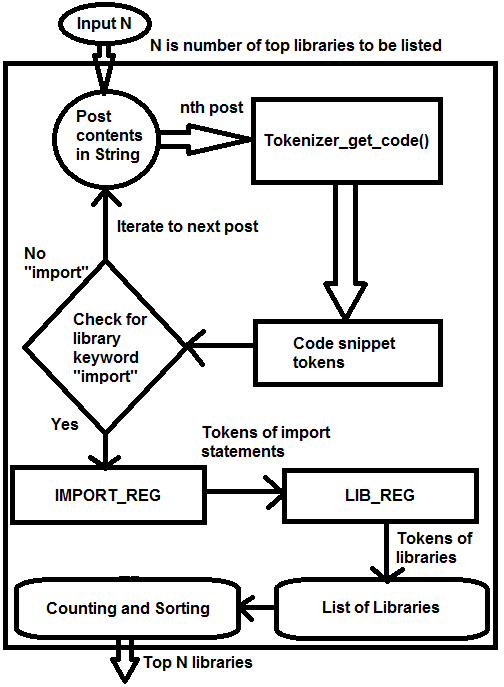
\includegraphics[width=0.9\linewidth]{application}
\caption{Implementation of \texttt{get\_libraries\,()}}\label{img:app}
\end{figure}

The top 10 most common libraries in the dataset are \texttt{numpy}, \texttt{re},
\texttt{sys}, \texttt{random}, \texttt{os}, \texttt{collections}, \texttt{time},
\texttt{pandas}, \texttt{csv} and \texttt{math}.

\section*{Appendix}

\subsection*{Individual Contributions}

The five members contribute \textbf{equally} to this project.

\subsection*{Project Structure and Documentation}

The file structure of this project is as follows:

\begin{lstlisting}
source_code/
    raw_data/
        query.sql               # SQL query
        QueryResults.csv        # raw data
                                  (1754 posts)
        TokenTagRaw.csv         # raw annotation data
                                  (100 posts)
        IrregularTokenSent.csv  # irregular tokens
                                  sentences (10)
    tagged_data/
        [100 tagged files]
        Annotation Notes.txt    # some annotation notes
    dataset.py
    stem_and_pos.py
    tokenizer.py
    test.py
    main.py                     # main calling script
report/
    [report materials]
\end{lstlisting}

Calling just the main script (by running \texttt{python source\_code\\/main.py})
would print out this command-line usage:

\begin{lstlisting}
$ python source_code/main.py
Invalid arguments! Exiting...
usage: main.py [report|stempos|test|eval|tokenize|
                irregular|commonX]
            report          report dataset stats
            stempos         stemming and POS tagging
                            on dataset
            test            test the tokenizer
            eval            evaluate the tokenizer
                            on annotated dataset
            tokenize        tokenize the dataset,
                            output irregular tokens
            irregular       POS tagging on sentences
                            with irregular tokens
            commonX         get the most common X
                            libraries from the dataset
\end{lstlisting}

\subsection*{Sample Project Runs}

Reporting of dataset statistics:

\begin{lstlisting}
$ python source_code/main.py report
Number of questions: 500
Number of answers: 1254
Average number of answers per questions: 2.508
Questions with 1 answer: 259
Questions with 2 answers: 107
Questions with 3 or more answers: 134
\end{lstlisting}

Stemming and POS tagging on the dataset (there are four separate print outputs
--- 10 random sentences, top 20 words before stemming, top 20 words after
stemming, the original words):

\begin{lstlisting}
$ python source_code/main.py stempos
[[('You', 'PRP'), ('are', 'VBP'), ('being', 'VBG'),
('tricked', 'VBN')...]]
[('', 20481), ('I', 947),...]]
[('', 20481), ('I', 947),...]]
[[''], ['I'], ...]]
\end{lstlisting}

Testing of the tokenizer:

\begin{lstlisting}
$ python3 source_code/main.py test
................................................
..........................
------------------------------------------------
Ran 74 tests in 0.010s

OK
\end{lstlisting}

Evaluating the tokenizer:

\begin{lstlisting}
$ python source_code/main.py eval
...
Id: 38810765, precision: 1.000, recall: 1.000, f1: 1.000
Id: 38834478, precision: 1.000, recall: 1.000, f1: 1.000
Id: 39432272, precision: 0.651, recall: 0.719, f1: 0.683
Id: 40488966, precision: 1.000, recall: 1.000, f1: 1.000
Id: 45003750, precision: 1.000, recall: 1.000, f1: 1.000
Overall: precision: 0.972, recall: 0.976, f1: 0.974
\end{lstlisting}

Outputting irregular tokens from the dataset:

\begin{lstlisting}
$ python source_code/main.py tokenize
Using Unix dictionary...
[..., ('Django', 64), ('app', 61)...]
\end{lstlisting}

POS tagging on sentences with irregular tokens:

\begin{lstlisting}
$python source_code/main.py irregular
[('I', 'PRP'), ("'m", 'VBP'), ('using', 'VBG'),
('Google', 'NNP'),...
\end{lstlisting}

Getting the most common libraries from the dataset:

\begin{lstlisting}
$ python source_code/main.py common5
[('numpy', 51), ('re', 32), ('sys', 29), ('random', 22),
('os', 22)]
$ python source_code/main.py common10
[('numpy', 51), ('re', 32), ('sys', 29), ('random', 22),
('os', 22), ('collections', 21), ('time', 18), ('pandas',
17), ('csv', 16), ('math', 14)]
\end{lstlisting}